\documentclass{article}
\usepackage[utf8]{inputenc}
\usepackage{graphicx}
\usepackage{geometry}
\geometry{a4paper, total={16cm, 24cm}, top=2cm}
\usepackage{amsmath}
\usepackage{blindtext}
\graphicspath{ {img/} }
\usepackage{listings}
\usepackage{color}
\usepackage{siunitx}
\usepackage{hyperref}
\hypersetup{
    colorlinks=true,
    linkcolor=blue,
    filecolor=magenta,      
    urlcolor=cyan,
    }
\definecolor{dkgreen}{rgb}{0,0.6,0}
\definecolor{gray}{rgb}{0.5,0.5,0.5}
\definecolor{mauve}{rgb}{0.58,0,0.82}

\lstset{ %frame=tb,
  language=C,
  aboveskip=3mm,
  belowskip=3mm,
  showstringspaces=false,
  columns=flexible,
  numbers=left,
  basicstyle={\small\ttfamily},
  numberstyle=\tiny\color{gray},
  keywordstyle=\color{blue},
  commentstyle=\color{dkgreen},
  stringstyle=\color{mauve},
  breaklines=true,
  breakatwhitespace=true,
  tabsize=3  
}


\title{Week 9 Programming Assignment}
\author{Steffen Petersen | au722120}
\date{November 7th 2022}

\begin{document}
%\tableofcontents

\maketitle
\vspace{5pt}
\noindent Here is the link for my repository, in which you will find all the edited code files and such.\\
\url{https://github.com/Aarhus-University-ECE/assignment-9-SirQuacc}
\section{}
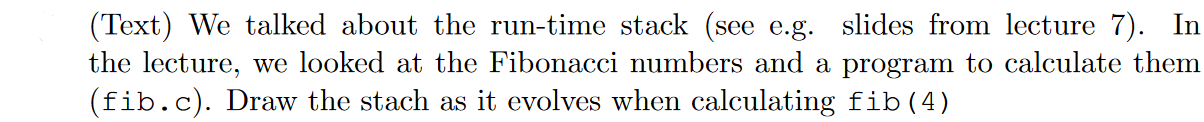
\includegraphics[width=\linewidth, keepaspectratio=true]{task1}
\vspace{2pt}\\
In the image below I've drawn a schematic of how the runtime stack evolves as the function calls upon itself. It will start returning
values to the previous functions once it reaches any base case, and a recursion branch ends. Each box
represents a new function call, i.e. a new stack in the runtime.
The timeline runs left to right.

\begin{center}
    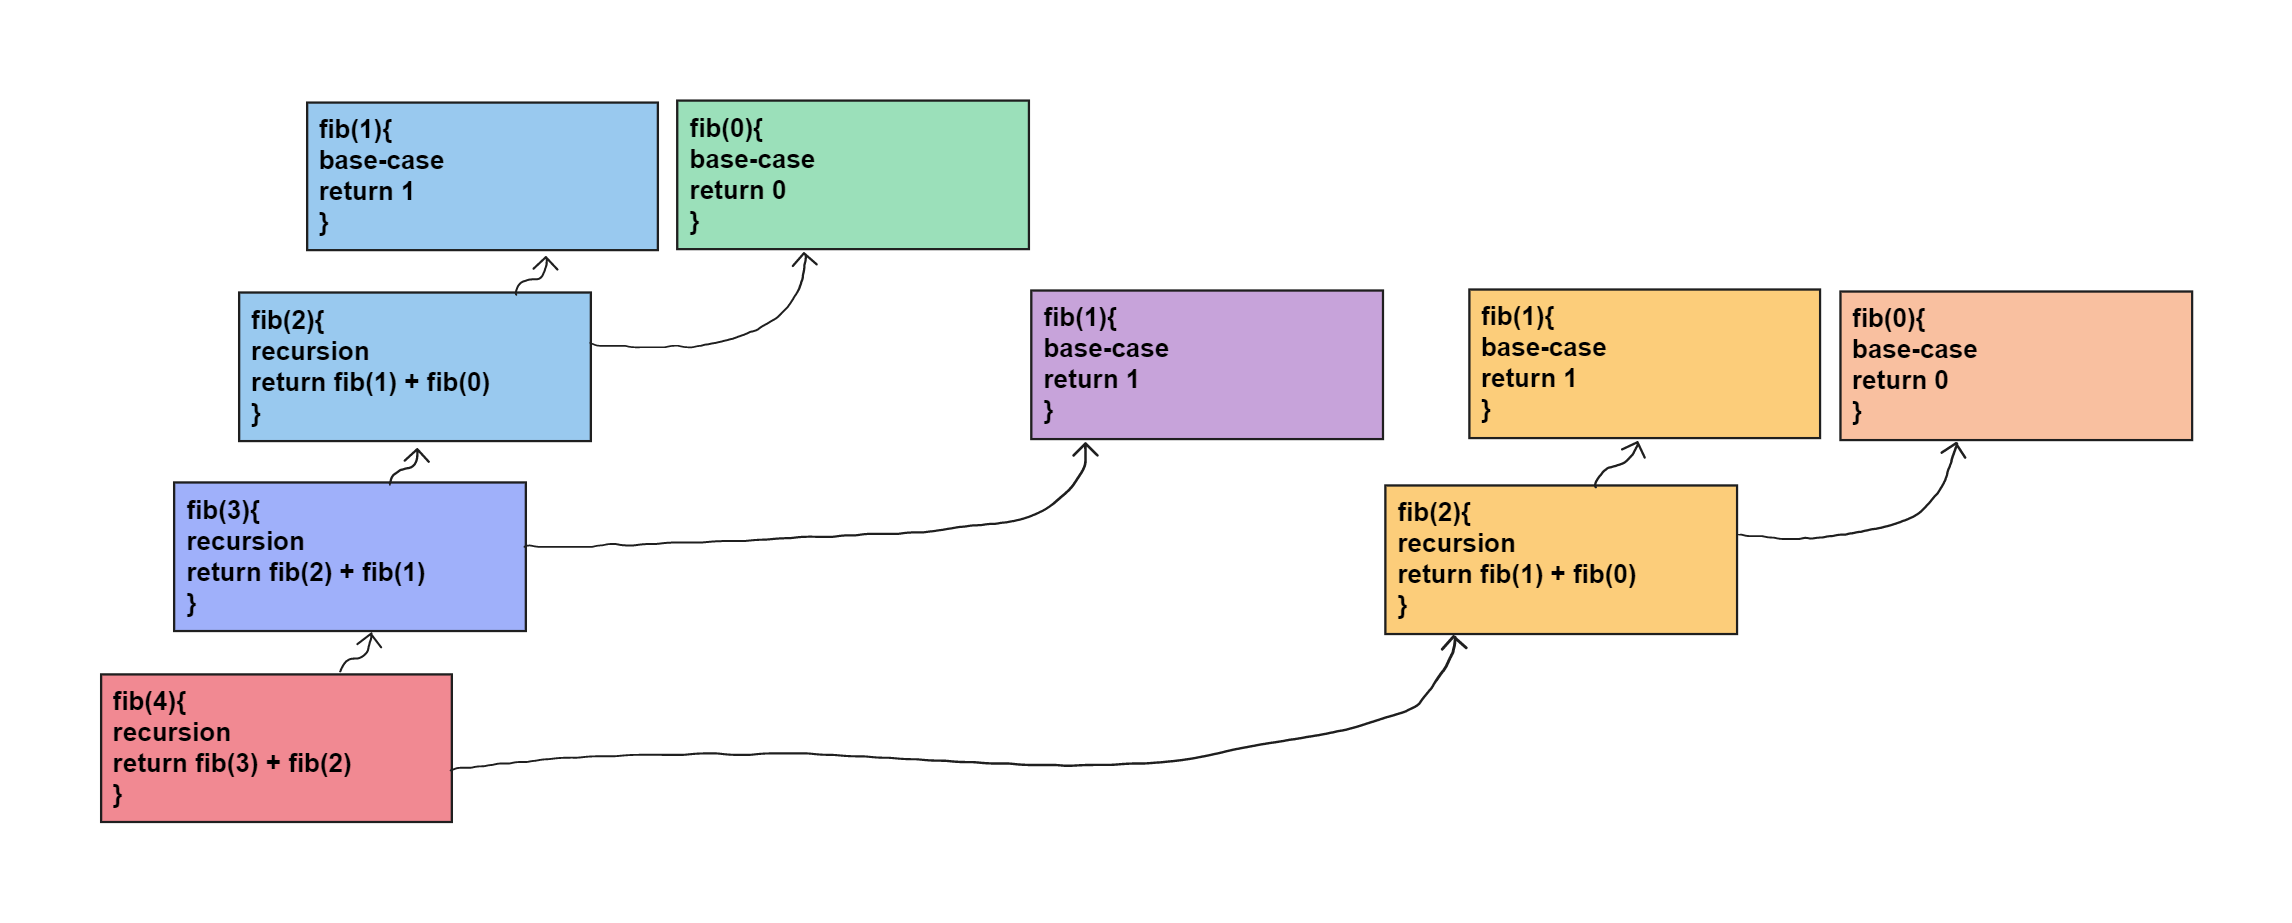
\includegraphics[width=0.95\linewidth, keepaspectratio=true]{runtimestack}
\end{center}

\pagebreak
\section{}
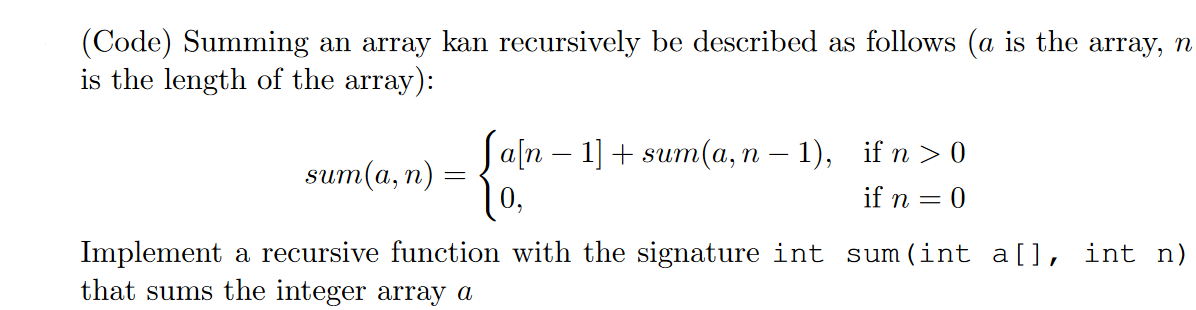
\includegraphics[width=\linewidth, keepaspectratio=true]{task2}
\vspace{2pt}
Below is the recursive function, it can also be found in sum.c
\begin{lstlisting}
    int sum(int a[], int n)
    {
        assert(!(n < 0)); // Can't search an array of lower than 0 length
        if(n == 0){
            return 0; //Base case, we're at the end of he array, return 0 as the "sum" of nothing
        }
        else return a[n-1] + sum(a, n-1); //Recursively ask for the sum of the next number, and add it to the current
    }
\end{lstlisting}


\section{}
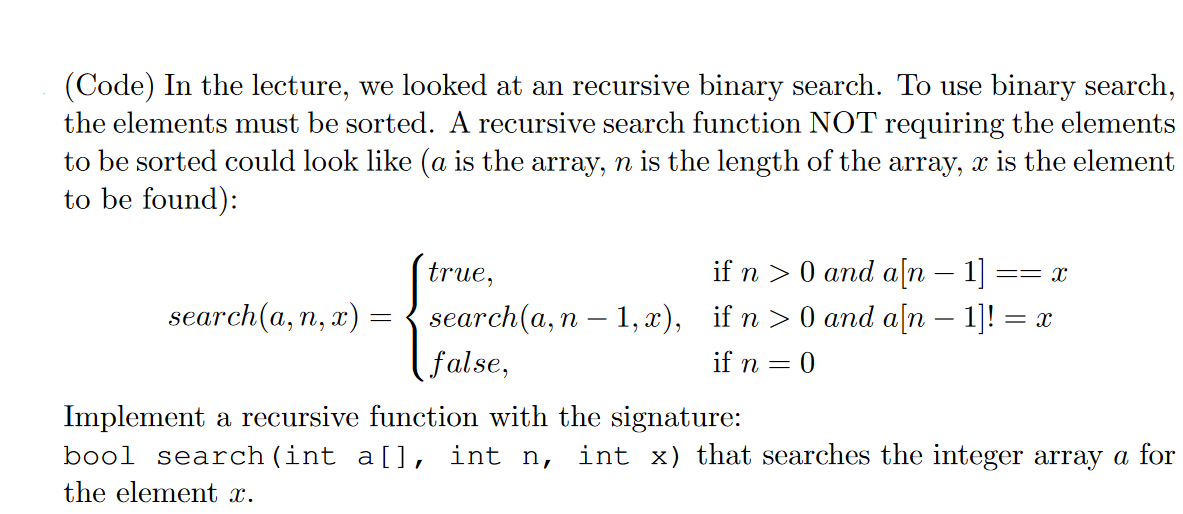
\includegraphics[width=\linewidth, keepaspectratio=true]{task3} 
The code is seen below and can be found in search.c
\begin{lstlisting}
    bool search(int a[], int n, int x)
    {
        assert(!(n < 0)); // Can't search an array of lower than 0 length
        if(n == 0){ //Base case, if we're beyond the array, element x wasn't in there,
            return false;
        }
        if(x == a[n-1]){ //Recusively check with linear search if x is equal to any element in the array of length n.
            return true;
        } else rethurn search(a, n-1, x);
    }
\end{lstlisting}
\vspace{1cm}

\pagebreak
\section{}
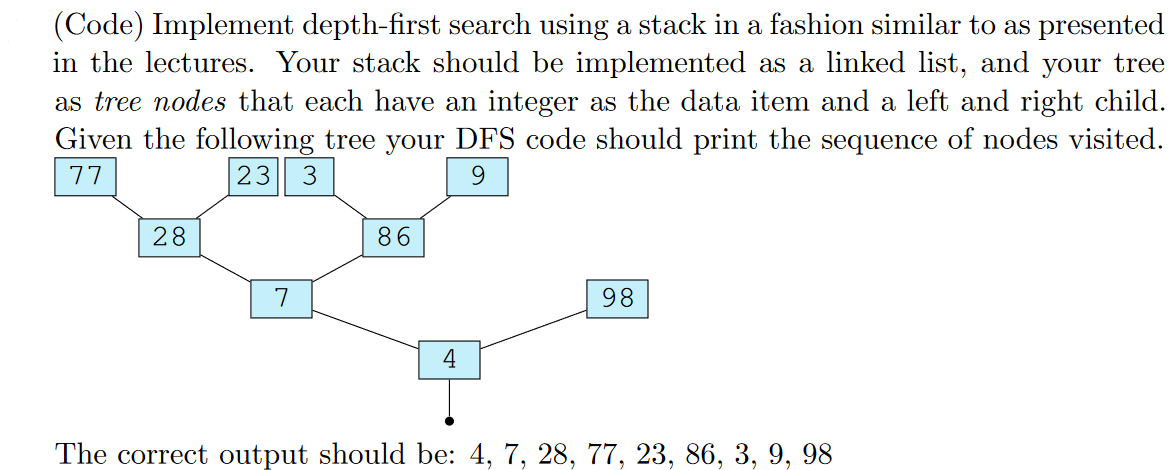
\includegraphics[width=\linewidth, keepaspectratio=true]{task4}
Below is my code for this function, it can also be found in dfs.c
\begin{lstlisting}
    void DFT (node * root)
    {
      printf("The given tree:\n");
      print_tree(root, 0); //Print the given tree first
    
      stack* mainStack = malloc(sizeof(stack)); //Allocate a stack node
      initStack(mainStack); //Initialize the stack
      mainStack = push(mainStack, root); //Push the root on to the stack first
      stack* popped; //Pointer to the saved node after popping
    
      printf("Order of visiting tree: ");
      while(!isEmpty(mainStack)){ //!isEmpty(mainStack)
        popped = pop(&mainStack); //Pop the top node, popped variable saves pointer to the popped node
        print_node(popped->node); //Print the visited (popped) node's value.
        if(popped->node->rchild != NULL) mainStack = push(mainStack, popped->node->rchild); //If there is a right child, add this to the stack
        if(popped->node->lchild != NULL) mainStack = push(mainStack, popped->node->lchild); //If there is a left child, add this to the stack
        free(popped); // Free stack-node, clean-up.
      }
      printf("\n");
    }
\end{lstlisting}


\vspace{2pt}


\end{document}